\subsubsection{Control de balanceo}

            A continuación se derivan las ecuaciones que modelan el sistema carro-pendulo. Se utilizará el metodo de Lagrange definiendo las cordenadas generalizadas 
            \(x_t\) y \(\theta\) . Donde \(x_t\) es la posición del carro y \(\theta\) es el angulo del pendulo respecto a la vertical. 
            A modo de simplificaion se toma \(l\) como un parametro y no como una funcion del tiempo.
            El sistema se modela siguiento el modelo físico de la figura 3 del enunciado.
            \begin{figure}[H]
                \centering
                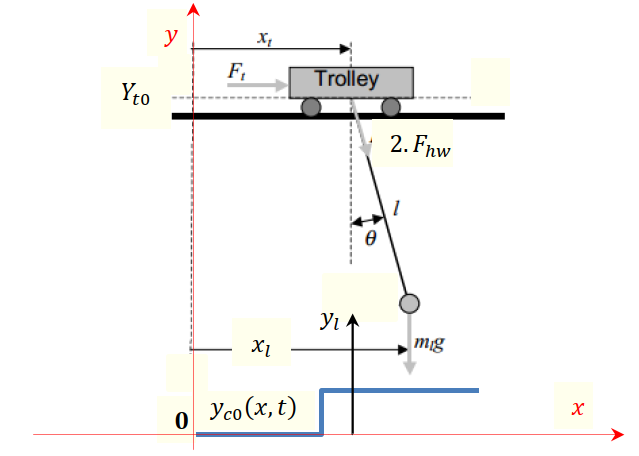
\includegraphics[width=0.5\textwidth]{figs/figure3_enunciado.png}
                \caption{Modelo físico simplificado del subsistema Carro – Cable – Carga y Perfil de Obstáculos}
                \label{fig:pendulo}
            \end{figure}
            
            \begin{equation}\label{eq:kinetic1}
                K = K_t + K_{lx} + K_{ly}
            \end{equation}
            \begin{equation}\label{eq:xl}
                x_l=x_t+l\sin{\theta}
            \end{equation}
            \begin{equation}\label{eq:dxl}
                \dot{x_l}=\dot{x_t}+l\cos{\theta}\dot{\theta}
            \end{equation}
            \begin{equation}\label{eq:y}
                y_l=Y_{t0}-l\cos{\theta}
            \end{equation}
            \begin{equation}\label{eq:dy}
                \dot{y_l}=-l\sin{\theta}\dot{\theta}
            \end{equation}

            \begin{equation}\label{eq:kinetic2}
                K = \frac{1}{2}m_t\dot{x_t}^2   +\frac{1}{2}m_l\dot{x_l}^2  +\frac{1}{2}m_l\dot{y_l}^2
            \end{equation}

            \begin{equation}\label{eq:kinetic3}
                K = \frac{1}{2}m_t\dot{x_t}^2   +\frac{1}{2}m_l(\dot{x_t}+l\cos{\theta}\dot{\theta})^2  +\frac{1}{2}m_l(-l\sin{\theta}\dot{\theta})^2
            \end{equation}

            \begin{equation}\label{eq:kinetic4}
                    K = \frac{1}{2}m_t\dot{x_t}^2 +\frac{1}{2}m_l(\dot{x_t}^2+l^2\cos^2{\theta}\dot{\theta}^2
                    +2l\dot{x_t}\cos{\theta}\dot{\theta})+\frac{1}{2}m_ll^2\sin^2{\theta}\dot{\theta}^2
            \end{equation}

            \begin{equation}\label{eq:potential}
                U = -m_lgl\cos{\theta}
            \end{equation}
            \begin{equation}\label{eq:lagrange}
                L = K - U
            \end{equation}

            \begin{equation}\label{eq:lagrange2}
                    L = \frac{1}{2}m_t\dot{x_t}^2
                    +\frac{1}{2}m_l(\dot{x_t}^2
                +l^2\cos^2{\theta}\dot{\theta}^2
                +2l\dot{x_t}\cos{\theta}\dot{\theta})
                +\frac{1}{2}m_ll^2\sin^2{\theta}\dot{\theta}^2
                +m_lgl\cos{\theta}
            \end{equation}

            \begin{equation}\label{eq:lagrange3}
                L = \frac{1}{2}m_t\dot{x_t}^2+\frac{1}{2}m_l\dot{x_t}^2
                +\frac{1}{2}m_ll^2\dot{\theta}^2
                +m_l\dot{x_t}l\cos{\theta}\dot{\theta}
                +m_lgl\cos{\theta}
            \end{equation}

            Se define el sistema de ecuaciones de Euler-Lagrange:
            \begin{equation}\label{eq:euler1}
                \frac{d}{dt}\left(\frac{\partial L}{\partial \dot{q}_i}\right)-\frac{\partial L}{\partial q_i}=Q_i
            \end{equation}

            Para \(q_i = x_t\):
            \begin{equation}\label{eq:euler2}
                \frac{d}{dt}\left(\frac{\partial L}{\partial \dot{x}_t}\right)-\frac{\partial L}{\partial x_t}=Q_t
            \end{equation}
            \begin{equation}
                \frac{\partial L}{\partial \dot{x}_t}= (m_t+m_l)\dot{x}_t+m_ll\cos{\theta}\dot{\theta}
            \end{equation}
            \begin{equation}            
                    \frac{d}{dt}\left(\frac{\partial L}{\partial \dot{x}_t}\right)= 
                    (m_t+m_l)\ddot{x}_t+m_ll\cos{\theta}\ddot{\theta}-m_ll\sin{\theta}\dot{\theta}^2
            \end{equation}
            \begin{equation}
                \frac{\partial L}{\partial x_t}=0
            \end{equation}
            Entonces:
            \begin{equation}
                (m_t+m_l)\ddot{x}_t+m_ll\cos{\theta}\ddot{\theta}-m_ll\sin{\theta}\dot{\theta}^2=F_t(t)-b_{eqt} \dot{x}_t
            \end{equation}

            Para \(q_i = \theta\):

            \begin{equation}\label{eq:euler3}
                \frac{d}{dt}\left(\frac{\partial L}{\partial \dot{\theta}}\right)-\frac{\partial L}{\partial \theta}=Q_{\theta}
            \end{equation}

            \begin{equation}
                \frac{\partial L}{\partial \dot{\theta}}=m_l\dot{x_t}l\cos{\theta}+m_ll^2\dot{\theta}
            \end{equation}

            \begin{equation}
                    \frac{d}{dt}\left(\frac{\partial L}{\partial \dot{\theta}}\right)= m_l\ddot{x_t}l\cos{\theta} -m_l\dot{x_t}l\sin{\theta}\dot{\theta}+m_ll^2\ddot{\theta}
            \end{equation}

            \begin{equation}
                \frac{\partial L}{\partial \theta}=-m_l\dot{x_t}l\sin{\theta}\dot{\theta}-m_lgl\sin{\theta}
            \end{equation}

            Entonces:
            \begin{equation}
                m_l\ddot{x_t}l\cos{\theta} -m_l\dot{x_t}l\sin{\theta}\dot{\theta}+m_ll^2\ddot{\theta}+m_l\dot{x_t}l\sin{\theta}\dot{\theta}+m_lgl\sin{\theta}=0
            \end{equation}

            Finalmente, el sistema de ecuaciones que define el modelo del sistema carro-pendulo es:
            \begin{equation}
                \begin{cases}
                    (m_t+m_l)\ddot{x}_t+m_ll\cos{\theta}\ddot{\theta}-m_ll\sin{\theta}\dot{\theta}^2=F_t(t)-b_{eqt} \dot{x}_t\\
                    m_l\ddot{x_t}l\cos{\theta} -m_l\dot{x_t}l\sin{\theta}\dot{\theta}+m_ll^2\ddot{\theta}+m_l\dot{x_t}l\sin{\theta}\dot{\theta}+m_lgl\sin{\theta}=0
                \end{cases}
            \end{equation}

            \begin{empheq}[box=\fbox]{equation}
                \begin{cases}
                    (m_t+m_l)\ddot{x}_t + m_l l \cos{\theta} \ddot{\theta} - m_l l \sin{\theta} \dot{\theta}^2 = 0 \\
                    \ddot{x}_t \cos{\theta} + l \ddot{\theta} + g \sin{\theta} = 0
                \end{cases}
            \end{empheq}


            Para representar lo en el espacio de estados se definen las siguientes variables de estado \(x\) y entradas \(u\):
            \begin{equation}
                x = \begin{bmatrix}
                    \theta \\
                    \dot{\theta}
                \end{bmatrix}
            \end{equation}
            \begin{equation}
                u = \ddot{x_l}
            \end{equation}

            Entonces, se obtiene el siguiente modelo en el espacio de estados no lineal:

            \begin{equation}
                \begin{cases}
                    \dot{x} = f(x,u,t) ; x(0) = x_0 \\
                    y = h(x,u,t)
                \end{cases}
            \end{equation}

            \begin{equation}
                \begin{cases}
                    ddot{\theta} = \ddot{\theta}
                    \ddot{\theta} = 
                \end{cases}